\documentclass[11pt]{article}
\pdfoutput=1

\usepackage{../../jcapmod}
\input{../../preamble}
\graphicspath{{figures/}}

% TikZ for inline figures
\usetikzlibrary{positioning, arrows.meta, shapes.geometric, fit, backgrounds, matrix, decorations.pathreplacing, calc}

\begin{document}
\thispagestyle{plain}

\newcommand{\nnicon}{%
\raisebox{-0.12ex}{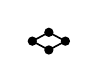
\begin{tikzpicture}[scale=1.4]
    % Simple network icon: three nodes connected
    \fill (0, 0) circle (1.2pt);
    \fill (0.15, 0.08) circle (1.2pt);
    \fill (0.15, -0.08) circle (1.2pt);
    \fill (0.3, 0) circle (1.2pt);
    \draw[line width=0.6pt] (0, 0) -- (0.15, 0.08);
    \draw[line width=0.6pt] (0, 0) -- (0.15, -0.08);
    \draw[line width=0.6pt] (0.15, 0.08) -- (0.3, 0);
    \draw[line width=0.6pt] (0.15, -0.08) -- (0.3, 0);
\end{tikzpicture}}%
}

\chapterheading{\nnicon\hspace{0.4em}$\cdot$ Neural Networks and Inductive Biases}

\vspace{1em}
\begin{quote}
\textit{``Look. The models, they just want to learn. You have to understand this. The models, they just want to learn.''}

\raggedleft-- Ilya Sutskever
\end{quote}
\vspace{0.5em}

\section{Modeling unknown functions}

Scientific data is full of relationships we can measure but not write down. A telescope records stellar spectra; the mapping from spectrum to stellar composition is complex. A detector measures particle interactions; extracting physical parameters requires inverting a complicated function. We have $(x, y)$ pairs and want to learn $y = f(x)$, but $f$ has no closed form.

\paragraph{The manifold hypothesis.} Scientific data is high-dimensional, but it's generated by low-dimensional processes. A cosmological density field has millions of voxels, but it's determined by just a handful of cosmological parameters ($\Omega_m$, $\sigma_8$, $H_0$, \ldots) plus initial conditions. A protein structure has thousands of atomic coordinates, but viable configurations are constrained by bond lengths, angles, and evolutionary pressures to a far smaller space.

This is the \emph{manifold hypothesis}: high-dimensional data concentrates near a lower-dimensional manifold embedded in the ambient space. The manifold isn't arbitrary---its geometry reflects the underlying science, and nearby on the manifold correspond to similar physical states.

Why does this help? Learning becomes tractable because we only need to model the manifold, not the full huge-dimensional space. The curse of dimensionality applies to the \emph{intrinsic} dimension (the manifold), not the \emph{ambient} dimension (e.g., the pixel space).

\paragraph{Summary statistics as projections.} Scientists have long exploited manifold structure through hand-crafted summary statistics. Consider a cosmological density field. The raw data is a 3D grid of densities---millions of numbers. But much of what we care about is captured by the \emph{power spectrum} $P(k)$: how much structure exists at each spatial scale.

The power spectrum is a projection from the high-dimensional data manifold to a lower-dimensional summary. It preserves certain information (the amplitude of fluctuations at each scale) while discarding other information (the phases---where exactly the structures are located). This is exactly what we want: \textbf{compress the data while retaining what matters for the scientific question we're asking}.
%
\emph{Many different data points can map to the same summary}. Infinitely many cosmological fields share the same power spectrum---they differ only in their phases. The summary defines equivalence classes on the manifold.

\begin{figure}[h]
\centering
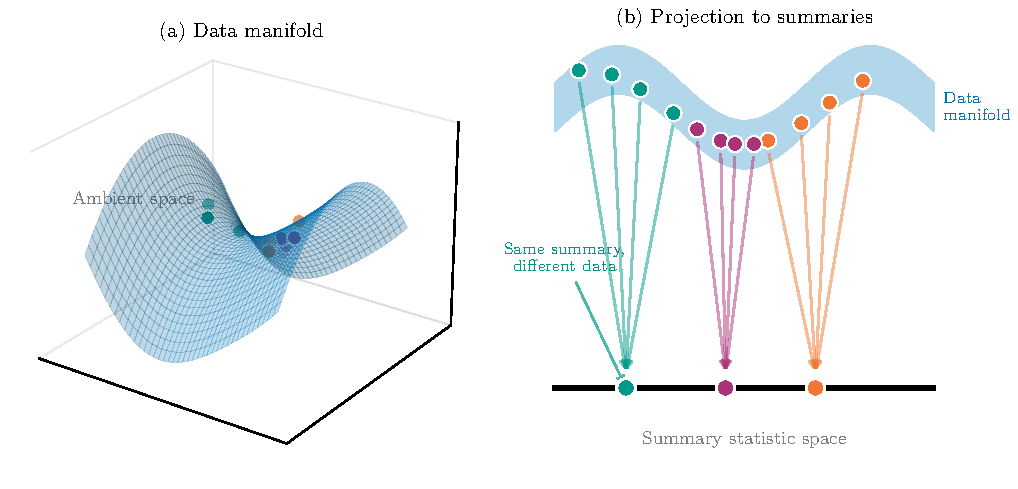
\includegraphics[width=\textwidth]{figures/manifold_and_summaries.pdf}
\caption{The manifold hypothesis and summary statistics. (a) Scientific data lives on a low-dimensional manifold embedded in high-dimensional ambient space. Points of the same color represent different configurations. (b) Summary statistics project the manifold to a lower-dimensional space. Multiple points on the manifold (same color) map to a single summary---these are equivalence classes of ``the same for my purposes.''}
\label{fig:manifold}
\end{figure}

\paragraph{Why summaries work.} Good summaries encode domain knowledge. The power spectrum is translation-invariant by construction---shifting the field doesn't change $P(k)$. The symmetry is built into the summary, so downstream models don't have to learn it.

But summaries have limits. The power spectrum captures Gaussian structure perfectly but misses higher-order correlations. Hand-crafted molecular fingerprints might miss subtle electronic effects. Compressing data is a trade-off!

\paragraph{Data-driven projections.} Can we learn summaries without domain expertise? PCA finds the linear projection that preserves the most variance---a data-driven approach that requires no physics knowledge. But PCA assumes the data manifold is flat. It finds the best hyperplane through the data, missing any curvature. When the manifold is nonlinear (as it usually is for complex scientific data), PCA captures only a shadow of the true structure. Other data-driven methods (t-SNE, UMAP, Isomap, \ldots) try to preserve local distances or neighborhood structure, but they too struggle with complex manifolds and scale poorly to large datasets.

\paragraph{Learning nonlinear projections.} Neural networks learn summaries from data. Instead of hand-crafting which aspects of the manifold to preserve, we parameterize a flexible family of projections and let optimization find what works for the task. The architecture encodes structural assumptions (\emph{inductive biases}) that constrain which projections are possible. Without them, we might need impossibly large datasets to discover structure that physics already tells us must be there.

\section{Neural networks: composing simple functions}

A neural network builds complex functions by composing simple ones. Apply a linear transformation, then a simple nonlinearity, then another linear transformation, and so on:
\begin{align}
h_1 &= \sigma(W_1 x + b_1) \\
h_2 &= \sigma(W_2 h_1 + b_2) \\
y &= W_3 h_2 + b_3
\end{align}
Each layer applies weights $W_\ell$, biases $b_\ell$, and a nonlinear activation $\sigma$. This is a \emph{multilayer perceptron} (MLP).

\begin{figure}[h]
\centering
\input{figures/mlp.tex}
\caption{A multilayer perceptron with two hidden layers. Each layer applies a linear transformation followed by a nonlinearity. All neurons in adjacent layers are connected (``fully connected'').}
\label{fig:mlp}
\end{figure}

Without $\sigma$, the network collapses to a single linear map:
\beq
W_2 (W_1 x + b_1) + b_2 = (W_2 W_1) x + (W_2 b_1 + b_2) = W' x + b'
\eeq
No matter how many layers, the result is linear. The nonlinearity is what gives depth its power.

\paragraph{What can nonlinearity do?} Consider the XOR problem: two classes arranged so no single line can separate them (Figure~\ref{fig:decision_boundary}). A linear model fails. But a network with one hidden layer can create a piecewise-linear decision boundary that correctly separates the classes. Adding more layers and neurons produces smoother, more complex boundaries.

\begin{figure}[h]
\centering
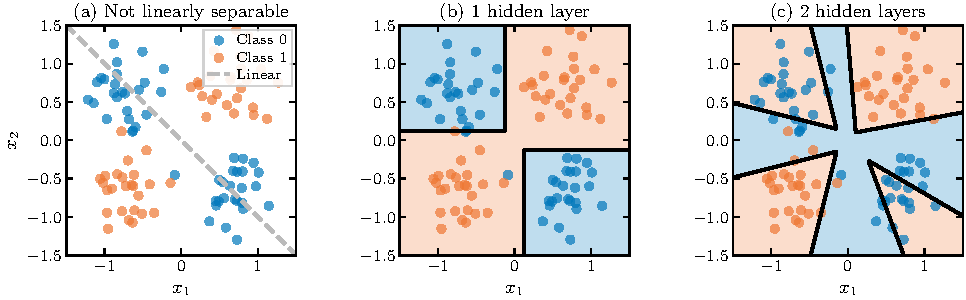
\includegraphics[width=\textwidth]{figures/nonlinear_decision_boundary.pdf}
\caption{Nonlinearity enables complex decision boundaries. (a) An XOR-like classification problem: no straight line separates the classes. (b) A single hidden layer creates a piecewise-linear boundary. (c) A deeper network produces a smooth boundary that perfectly separates the data.}
\label{fig:decision_boundary}
\end{figure}

\paragraph{Common activations.} The most common is ReLU, which is piecewise linear: identity for positive inputs, zero otherwise.

\beq
\sigma(z) = \max(0, z)
\eeq

\paragraph{Universal approximation.} With enough neurons, an MLP can approximate any continuous function. This is reassuring but not really of any practical use---it says nothing about how many parameters we need or whether we can find them by training.

%%%%%%%%%%%%%%%%%%%%%%%%%%%%%%%%%%%%%%%%%%%%%%%%%%%%%%%%%%%%%%%%%%
\section{Training deep networks}
%%%%%%%%%%%%%%%%%%%%%%%%%%%%%%%%%%%%%%%%%%%%%%%%%%%%%%%%%%%%%%%%%%

Deeper networks can represent more complex functions, but they're harder to train. Gradients must flow backward through many layers; they can vanish (shrink to zero) or explode (grow unboundedly). Two techniques make deep training possible: \textbf{residual connections} and \textbf{normalization}.

\paragraph{Residual connections.} Instead of learning $h' = F(h)$, learn the \emph{residual} $h' = F(h) + h$. The network learns what to \emph{add} to the input rather than computing the output from scratch.

\begin{figure}[h]
\centering
\input{figures/residual_connection.tex}
\caption{Residual (skip) connections. Left: a standard network computes $F(x)$. Right: a residual block computes $F(x) + x$. The skip connection provides a direct path for gradients, enabling training of very deep networks.}
\label{fig:residual}
\end{figure}

Why does this help? Gradients can flow directly through the skip connection, bypassing the layers entirely. Even if $F$ contributes small gradients, the identity path ensures signal reaches early layers.

\paragraph{Normalization.} During training, the distribution of each layer's inputs shifts as earlier layers change. \emph{Batch normalization} fixes this by normalizing each feature across the mini-batch to zero mean and unit variance. \emph{Layer normalization} normalizes across features for each sample independently (standard in Transformers). Both smooth the loss landscape and reduce sensitivity to initialization.

\paragraph{The modern recipe.} Nearly all successful deep networks use both:
\beq
h' = h + F(\text{Norm}(h))
\eeq
First normalize, then apply the learned transformation $F$, then add the residual. This combination enables training networks with hundreds of layers.

\paragraph{Optimization.} We train by minimizing a loss function $\mathcal{L}(\theta)$ over parameters $\theta$. Standard gradient descent computes the gradient over the entire dataset and steps downhill:
\beq
\theta \leftarrow \theta - \eta \nabla_\theta \mathcal{L}
\eeq
The problem: gradient descent is deterministic. Where you end up depends entirely on where you start. If you initialize in the wrong ``valley'' of the loss landscape, you descend to a local minimum and stay there.

\emph{Stochastic gradient descent} (SGD) fixes this by adding noise. Instead of computing the gradient over all data, we use a random subset---a \emph{mini-batch}---at each step. The gradient estimate is noisy: it points roughly downhill, but not exactly. This noise lets SGD escape shallow local minima. A step might go temporarily uphill, hopping from one valley to another. On average we descend, but the stochasticity explores the landscape. \emph{Adam} and related optimizers adapt the learning rate per-parameter, using running estimates of gradient moments. Adam is often more robust to hyperparameter choices, making it a good default.

\paragraph{Batch size.} Mini-batch size controls the noise level. Larger batches give more accurate gradient estimates---less noise, more direct descent. Smaller batches add more noise, helping escape bad minima but making optimization noisier. There's evidence that the noise from small batches acts as implicit regularization, finding flatter minima that generalize better.

\begin{figure}[h]
\centering
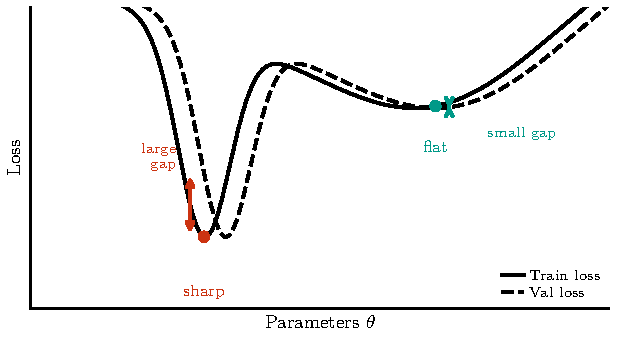
\includegraphics[width=0.65\textwidth]{figures/flat_minima.pdf}
\caption{Why flat minima generalize better. The validation loss landscape (dashed) is slightly shifted from training (solid). At a sharp minimum, this shift causes a large generalization gap. At a flat minimum, the same shift produces a much smaller gap---the solution is robust to distribution shift.}
\label{fig:flat_minima}
\end{figure}

\section{Autoencoders: learning to compress}

Supervised learning requires labels. But labels are expensive, and much scientific data is unlabeled. Can we learn useful representations without supervision?

\paragraph{The autoencoder idea.} Train a network to reconstruct its input. This seems trivial---just learn the identity function. The trick is to force the data through a \emph{bottleneck}: a low-dimensional intermediate representation.

\begin{figure}[h]
\centering
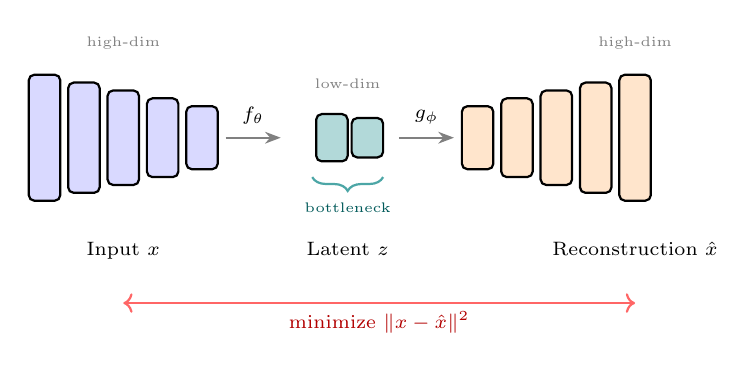
\begin{tikzpicture}[
    node distance=0.5cm,
    layer/.style={rectangle, draw, rounded corners=2pt, minimum width=0.4cm, thick},
    arrow/.style={-{Stealth[length=2mm]}, thick, gray},
    label/.style={font=\scriptsize},
    latent/.style={rectangle, draw, rounded corners=2pt, minimum width=0.4cm, fill=teal!30, thick}
]

% Input
\foreach \i/\h in {1/1.6, 2/1.4, 3/1.2, 4/1.0, 5/0.8} {
    \node[layer, fill=blue!15, minimum height=\h cm] (in\i) at (\i*0.5, 0) {};
}
\node[below=0.3cm, font=\scriptsize] at (1.5, -0.9) {Input $x$};
\node[above=0.1cm, font=\tiny, text=gray] at (1.5, 0.9) {high-dim};

% Encoder arrow
\draw[arrow] (2.8, 0) -- (3.5, 0);
\node[above=0.05cm, font=\scriptsize] at (3.15, 0) {$f_\theta$};

% Latent (bottleneck)
\foreach \i/\h in {1/0.6, 2/0.5} {
    \pgfmathsetmacro{\xpos}{3.7 + \i*0.45}
    \node[latent, minimum height=\h cm] (lat\i) at (\xpos, 0) {};
}
\node[below=0.3cm, font=\scriptsize] at (4.35, -0.9) {Latent $z$};
\node[above=0.1cm, font=\tiny, text=gray] at (4.35, 0.4) {low-dim};

% Decoder arrow
\draw[arrow] (5.0, 0) -- (5.7, 0);
\node[above=0.05cm, font=\scriptsize] at (5.35, 0) {$g_\phi$};

% Output (reconstruction) - mirrored to show expansion
\foreach \i/\h in {1/0.8, 2/1.0, 3/1.2, 4/1.4, 5/1.6} {
    \pgfmathsetmacro{\xpos}{5.5 + \i*0.5}
    \node[layer, fill=orange!20, minimum height=\h cm] (out\i) at (\xpos, 0) {};
}
\node[below=0.3cm, font=\scriptsize] at (8.0, -0.9) {Reconstruction $\hat{x}$};
\node[above=0.1cm, font=\tiny, text=gray] at (8.0, 0.9) {high-dim};

% Loss annotation
\draw[<->, thick, red!60] (1.5, -2.1) -- (8.0, -2.1);
\node[font=\scriptsize, text=red!70!black] at (4.75, -2.35) {minimize $\|x - \hat{x}\|^2$};

% Bottleneck annotation
\draw[decorate, decoration={brace, amplitude=5pt, mirror}, thick, teal!70]
    (3.9, -0.5) -- (4.8, -0.5);
\node[font=\tiny, text=teal!70!black, below=0.15cm] at (4.35, -0.55) {bottleneck};

\end{tikzpicture}
b
\caption{Autoencoder architecture. The encoder $f_\theta$ compresses high-dimensional input to a low-dimensional latent representation $z$. The decoder $g_\phi$ reconstructs the input from $z$. The bottleneck forces the network to learn which information matters.}
\label{fig:autoencoder}
\end{figure}

The encoder $f_\theta: \R^D \to \R^d$ maps input $x$ to a low-dimensional latent code $z = f_\theta(x)$. The decoder $g_\phi: \R^d \to \R^D$ reconstructs the input: $\hat{x} = g_\phi(z)$. Train by minimizing reconstruction error:
\beq
\mathcal{L} = \|x - g_\phi(f_\theta(x))\|^2
\eeq
If $d \ll D$, the network can't memorize inputs---it must learn to compress. The latent space $z$ captures whatever structure is needed for reconstruction.

\paragraph{Connection to the manifold hypothesis.} Remember: data lives on a low-dimensional manifold. The autoencoder learns to find it. The encoder projects data onto the manifold (approximately); the decoder maps back to the ambient space. The latent dimension $d$ is a hypothesis about the manifold's intrinsic dimension.

If $d$ is too small, reconstruction suffers---you've lost information. If $d$ is too large, the network might not learn meaningful compression. In practice, you can tune $d$ or let the network learn sparsity through regularization.

The latent space often captures interpretable structure. An autoencoder trained on galaxy images might learn latents corresponding to size, brightness, and morphology---without ever being told these concepts exist. The network discovers the factors of variation that matter for reconstruction.

This makes autoencoders useful for dimensionality reduction---The latent $z$ is a compressed representation, like PCA but nonlinear---and e.g. anomaly detection. Data far from the training manifold reconstructs poorly; high reconstruction error flags anomalies. They can also denoise data by training on corrupted inputs and reconstructing clean outputs.

\paragraph{Limitations and extensions.} Standard autoencoders give you a latent space, but it may be irregular---points don't interpolate smoothly, and you can't easily sample new data. Variational autoencoders (VAEs) address this by imposing probabilistic structure on the latent space, enabling smooth interpolation and generation of new samples. We'll return to this when we discuss generative models.

%%%%%%%%%%%%%%%%%%%%%%%%%%%%%%%%%%%%%%%%%%%%%%%%%%%%%%%%%%%%%%%%%%
\section{Matching architecture to data structure}
%%%%%%%%%%%%%%%%%%%%%%%%%%%%%%%%%%%%%%%%%%%%%%%%%%%%%%%%%%%%%%%%%%

Fully connected networks treat every input dimension as unrelated. For an image, pixel $(0,0)$ has no special relationship to pixel $(0,1)$, even though they're neighbors. The network must learn from scratch that nearby pixels are correlated, that patterns can appear anywhere, that a galaxy in the corner is the same as one in the center.

With enough data, a fully connected network can learn this. But it's inefficient---we're asking the network to rediscover structure we already know. Scientific datasets can be limited in size, and sample efficiency matters---often better to build known structure into the architecture.

The rest of this chapter develops architectures for different data types:
\begin{center}
\begin{tabular}{lll}
\toprule
\textbf{Data type} & \textbf{Architecture} & \textbf{Inductive bias} \\
\midrule
Images/grids & CNN & Translation invariance + locality \\
Sequences & RNN & Temporal order \\
Sets & Deep Sets & Permutation invariance \\
Graphs & GNN & Permutation invariance + edges \\
\bottomrule
\end{tabular}
\end{center}

%%%%%%%%%%%%%%%%%%%%%%%%%%%%%%%%%%%%%%%%%%%%%%%%%%%%%%%%%%%%%%%%%%
\subsection{Grids $\to$ CNNs}

Images have two properties that fully connected networks ignore:
\begin{itemize}
    \item \textbf{Translation invariance}: An edge is an edge, regardless of where it appears. A galaxy in the corner should be classified the same as one in the center.
    \item \textbf{Locality}: To understand a pixel, look at its neighbors. Distant pixels are (initially) irrelevant. Global structure emerges from composing local features.
\end{itemize}
These assumptions reflect the physics of spatial data. The inductive bias is that patterns are local and can appear anywhere.

\paragraph{Deriving convolutions.} Start with a fully connected layer:
\beq
h_{ij} = \sum_{k,l} W_{ijkl} \, x_{kl}
\eeq
Weights $W_{ijkl}$ connect input position $(k,l)$ to output position $(i,j)$. For a megapixel image, this requires $10^{12}$ parameters.

\emph{Impose translation invariance}: The same pattern should be detected identically everywhere. Weights cannot depend on absolute position---only on the offset. Let $a = k - i$, $b = l - j$:
\beq
W_{ijkl} = W_{ab} \quad \Rightarrow \quad h_{ij} = \sum_{a,b} W_{ab} \, x_{i+a, j+b}
\eeq
This is a \emph{convolution}. The same small set of weights (a \emph{kernel}) slides across the image, computing the same operation at every position.

\emph{Impose locality}: Only look at nearby pixels. Restrict to a small window:
\beq
h_{ij} = \sum_{|a| \leq k} \sum_{|b| \leq k} W_{ab} \, x_{i+a, j+b}
\eeq
A $3 \times 3$ kernel has 9 parameters. We've gone from $10^{12}$ to 9---while encoding exactly the structure spatial data has.

\begin{figure}[h]
\centering
\input{figures/convolution.tex}
\caption{Convolution: a small kernel slides across the image, computing a weighted sum at each position. The same 9 weights are used everywhere (weight sharing). This kernel detects horizontal edges.}
\label{fig:convolution}
\end{figure}

\paragraph{What convolutions learn.} Each kernel extracts a local pattern. A horizontal edge detector:
\beq
\begin{pmatrix}
-1 & -1 & -1 \\
0 & 0 & 0 \\
+1 & +1 & +1
\end{pmatrix}
\eeq
This computes the difference between rows below and above---large where there's a horizontal intensity change. In a CNN, kernels are \emph{learned}. The network discovers which local patterns are useful for the task.

\paragraph{Channels.} A single kernel detects one pattern. To detect multiple patterns, use multiple kernels in parallel. Each kernel produces one \emph{output channel}---a feature map detecting that pattern across the image. A layer might have 64 or 256 channels, each detecting a different pattern.

The input can also have multiple channels: RGB images have 3 input channels; scientific images might have spectral bands or multiple observables. Each output channel combines information from all input channels:
\beq
h_{ij}^{(c)} = \sum_{c'} \sum_{a,b} W_{ab}^{(c,c')} \, x_{i+a, j+b}^{(c')}
\eeq
The kernel $W^{(c,c')}$ maps input channel $c'$ to output channel $c$. For a $3 \times 3$ kernel with 64 input and 128 output channels, this is $3 \times 3 \times 64 \times 128 \approx 74{,}000$ parameters---still far fewer than a fully connected layer.

\paragraph{Building hierarchies.} Stacking convolutional layers builds a hierarchy of features. Early layers detect simple patterns like edges and gradients; later layers combine these into textures, shapes, and eventually objects. Each layer's \emph{receptive field}---the input region affecting one output---grows with depth. After several layers, each output unit ``sees'' a large region of the input.

\begin{figure}[h]
\centering
\input{figures/cnn_hierarchy.tex}
\caption{Hierarchical feature learning in CNNs. Early layers detect simple patterns (edges), later layers detect complex structures (objects). Receptive field grows with depth; spatial resolution decreases.}
\label{fig:cnn_hierarchy}
\end{figure}

\emph{Pooling} (taking the max or average over small windows) downsamples spatial dimensions, reducing computation and building robustness to small translations.

CNNs are the standard tool for any data on a grid: images (galaxy classification, medical imaging), spectra (stellar spectra, mass spectra), spatial fields (climate data, cosmological density fields). The same architecture that recognizes cats recognizes spiral galaxies---the inductive bias (translation invariance, locality) matches the data structure.

%%%%%%%%%%%%%%%%%%%%%%%%%%%%%%%%%%%%%%%%%%%%%%%%%%%%%%%%%%%%%%%%%%
\subsection{Sequences $\to$ RNNs}
%%%%%%%%%%%%%%%%%%%%%%%%%%%%%%%%%%%%%%%%%%%%%%%%%%%%%%%%%%%%%%%%%%

Much scientific data is \emph{sequential}: time series, trajectories, genetic sequences. The inductive bias: order matters, and what happens now depends on what came before.

\paragraph{The idea.} Process the sequence one element at a time, maintaining a \emph{hidden state} $h_t$ that summarizes what we've seen so far:
\beq
h_t = \sigma(W_h h_{t-1} + W_x x_t + b)
\eeq
This is a \textbf{recurrent neural network} (RNN). The same function is applied at every timestep---weight sharing across time, analogous to weight sharing across space in CNNs.

\begin{figure}[h]
\centering
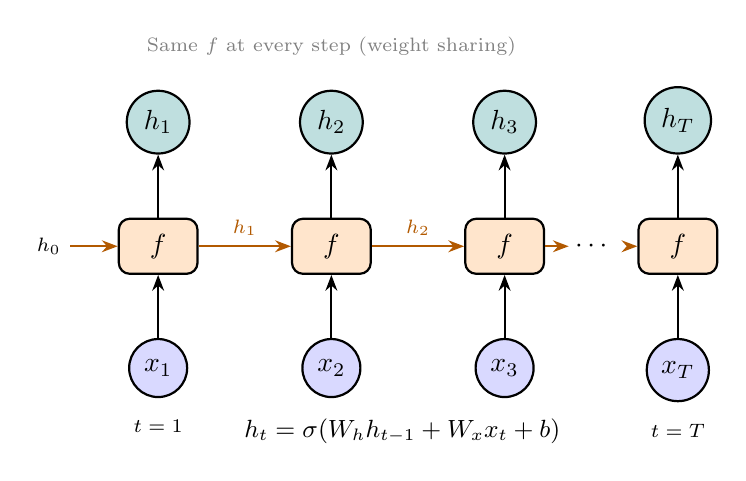
\begin{tikzpicture}[
    node distance=1.2cm,
    cell/.style={rectangle, draw, rounded corners, minimum width=1.0cm, minimum height=0.7cm, thick, fill=orange!20},
    input/.style={circle, draw, minimum size=0.6cm, fill=blue!15, thick},
    output/.style={circle, draw, minimum size=0.6cm, fill=teal!25, thick},
    arrow/.style={-{Stealth[length=2mm]}, thick},
    harrow/.style={arrow, orange!70!black},
    label/.style={font=\scriptsize}
]

% RNN cells
\node[cell] (rnn1) at (0, 0) {$f$};
\node[cell] (rnn2) at (2.2, 0) {$f$};
\node[cell] (rnn3) at (4.4, 0) {$f$};
\node[cell] (rnn4) at (6.6, 0) {$f$};

% Inputs
\node[input, below=0.8cm of rnn1] (x1) {$x_1$};
\node[input, below=0.8cm of rnn2] (x2) {$x_2$};
\node[input, below=0.8cm of rnn3] (x3) {$x_3$};
\node[input, below=0.8cm of rnn4] (x4) {$x_T$};

\draw[arrow] (x1) -- (rnn1);
\draw[arrow] (x2) -- (rnn2);
\draw[arrow] (x3) -- (rnn3);
\draw[arrow] (x4) -- (rnn4);

% Hidden states above
\node[output, above=0.8cm of rnn1] (h1) {$h_1$};
\node[output, above=0.8cm of rnn2] (h2) {$h_2$};
\node[output, above=0.8cm of rnn3] (h3) {$h_3$};
\node[output, above=0.8cm of rnn4] (h4) {$h_T$};

\draw[arrow] (rnn1) -- (h1);
\draw[arrow] (rnn2) -- (h2);
\draw[arrow] (rnn3) -- (h3);
\draw[arrow] (rnn4) -- (h4);

% Horizontal connections (hidden state flow)
\draw[harrow] (rnn1) -- node[above, font=\scriptsize] {$h_1$} (rnn2);
\draw[harrow] (rnn2) -- node[above, font=\scriptsize] {$h_2$} (rnn3);

% Dots between rnn3 and rnn4
\node at (5.5, 0) {$\cdots$};
\draw[harrow] (rnn3.east) -- ++(0.3, 0);
\draw[harrow] (6.0, 0) -- (rnn4.west);

% Initial hidden state
\node[left=0.6cm of rnn1, font=\scriptsize] (h0) {$h_0$};
\draw[harrow] (h0) -- (rnn1);

% Labels
\node[label, below=0.15cm of x1] {$t=1$};
\node[label, below=0.15cm of x4] {$t=T$};

% Shared weights annotation
\node[above=0.3cm of h2, font=\scriptsize, text=gray] {Same $f$ at every step (weight sharing)};

% Equation
\node[below=1.7cm of rnn2, xshift=0.9cm, font=\small] {
$h_t = \sigma(W_h h_{t-1} + W_x x_t + b)$
};

\end{tikzpicture}

\caption{A recurrent neural network unrolled through time. The same function (with shared weights) processes each input $x_t$ and the previous hidden state $h_{t-1}$ to produce the next hidden state $h_t$. The final state $h_T$ summarizes the entire sequence.}
\label{fig:rnn}
\end{figure}

\paragraph{The trouble with RNNs.} To learn from long sequences, gradients must flow backward through many timesteps, each multiplying by $W_h$. If $\|W_h\| < 1$, gradients shrink exponentially (\emph{vanishing gradients})---the network forgets distant inputs. Gated architectures (LSTMs, GRUs) add learned gates that control information flow, helping gradients propagate. But even with gating, RNNs process sequences \emph{sequentially}---you can't compute $h_{100}$ without first computing $h_1$ through $h_{99}$.

\paragraph{Beyond RNNs.} Transformers process all positions in parallel using attention (discussed later). They've largely replaced RNNs for most sequence tasks.

%%%%%%%%%%%%%%%%%%%%%%%%%%%%%%%%%%%%%%%%%%%%%%%%%%%%%%%%%%%%%%%%%%
\subsection{Sets and graphs $\to$ Deep Sets and GNNs}
%%%%%%%%%%%%%%%%%%%%%%%%%%%%%%%%%%%%%%%%%%%%%%%%%%%%%%%%%%%%%%%%%%

Much scientific data has relational structure: a molecule is atoms connected by bonds, a protein is residues along a backbone, a physical system is particles interacting pairwise. These are \emph{graphs}: nodes (entities) and edges (relationships). The structure is irregular---no grid, no canonical ordering.

The key symmetry: \textbf{permutation invariance}. Relabeling nodes (e.g., calling atom 1 ``atom 2'' instead) shouldn't change the output. This is the inductive bias for relational data.

\paragraph{Sets.} Before graphs, consider a \emph{set}---elements with no relationships. A point cloud. A bag of features. How do we build a function $f(\{x_1, \ldots, x_n\})$ that is invariant to ordering?

\paragraph{The Deep Sets theorem.} Any permutation-invariant function can be written as:
\beq
f(\{x_1, \ldots, x_n\}) = \rho\left( \sum_{i=1}^n \phi(x_i) \right)
\eeq
where $\phi$ processes each element independently and $\rho$ processes the aggregated result. This is the minimal architecture that respects the symmetry of sets.


\begin{figure}[h]
\centering
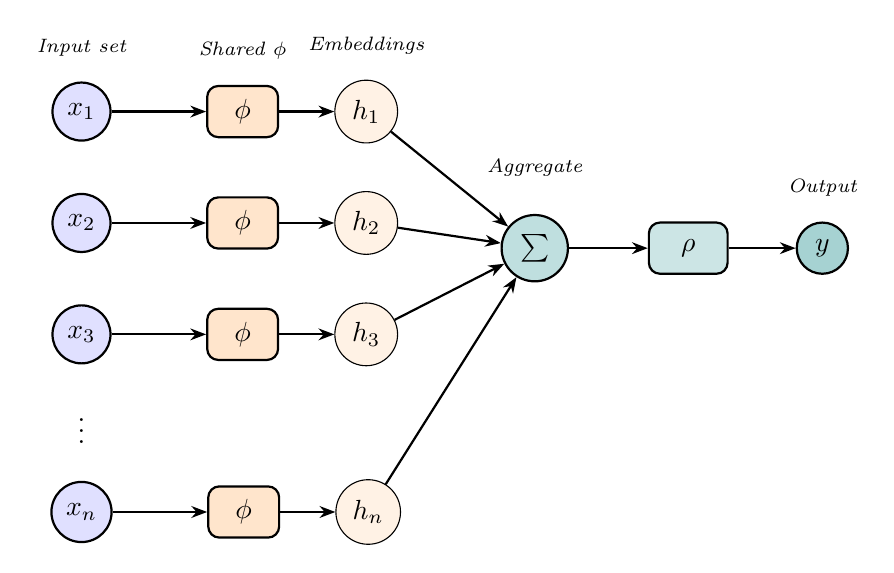
\begin{tikzpicture}[
    node distance=1.0cm and 1.3cm,
    element/.style={circle, draw, minimum size=0.7cm, fill=blue!12, thick},
    phi/.style={rectangle, draw, rounded corners, minimum width=0.9cm, minimum height=0.65cm, fill=orange!20, thick},
    hidden/.style={circle, draw, minimum size=0.55cm, fill=orange!10},
    sum/.style={circle, draw, minimum size=0.8cm, fill=teal!25, thick, font=\normalsize},
    rho/.style={rectangle, draw, rounded corners, minimum width=1.0cm, minimum height=0.65cm, fill=teal!20, thick},
    output/.style={circle, draw, minimum size=0.65cm, fill=teal!35, thick},
    arrow/.style={-{Stealth[length=2mm]}, thick},
    label/.style={font=\scriptsize\itshape}
]

% Input elements
\node[element] (x1) {$x_1$};
\node[element, below=0.65cm of x1] (x2) {$x_2$};
\node[element, below=0.65cm of x2] (x3) {$x_3$};
\node[below=0.35cm of x3, font=\normalsize] (dots) {$\vdots$};
\node[element, below=0.35cm of dots] (xn) {$x_n$};

% Phi networks (shared weights)
\node[phi, right=1.2cm of x1] (phi1) {$\phi$};
\node[phi, right=1.2cm of x2] (phi2) {$\phi$};
\node[phi, right=1.2cm of x3] (phi3) {$\phi$};
\node[phi, right=1.2cm of xn] (phin) {$\phi$};

% Hidden representations
\node[hidden, right=0.7cm of phi1] (h1) {$h_1$};
\node[hidden, right=0.7cm of phi2] (h2) {$h_2$};
\node[hidden, right=0.7cm of phi3] (h3) {$h_3$};
\node[hidden, right=0.7cm of phin] (hn) {$h_n$};

% Sum node
\node[sum, right=1.3cm of h2, yshift=-0.32cm] (sum) {$\sum$};

% Rho network
\node[rho, right=1.0cm of sum] (rho) {$\rho$};

% Output
\node[output, right=0.85cm of rho] (out) {$y$};

% Arrows from inputs to phi
\draw[arrow] (x1) -- (phi1);
\draw[arrow] (x2) -- (phi2);
\draw[arrow] (x3) -- (phi3);
\draw[arrow] (xn) -- (phin);

% Arrows from phi to hidden
\draw[arrow] (phi1) -- (h1);
\draw[arrow] (phi2) -- (h2);
\draw[arrow] (phi3) -- (h3);
\draw[arrow] (phin) -- (hn);

% Arrows from hidden to sum
\draw[arrow] (h1) -- (sum);
\draw[arrow] (h2) -- (sum);
\draw[arrow] (h3) -- (sum);
\draw[arrow] (hn) -- (sum);

% Arrow from sum to rho
\draw[arrow] (sum) -- (rho);

% Arrow from rho to output
\draw[arrow] (rho) -- (out);

% Labels
\node[label, above=0.2cm of x1] {Input set};
\node[label, above=0.2cm of phi1] {Shared $\phi$};
\node[label, above=0.2cm of h1] {Embeddings};
\node[label, above=0.35cm of sum] {Aggregate};
\node[label, above=0.2cm of out] {Output};

\end{tikzpicture}

\caption{Deep Sets architecture. Each element $x_i$ passes through the same network $\phi$ (weight sharing). Embeddings are summed (a symmetric operation), then processed by $\rho$ to produce the output. Reordering the inputs doesn't change the sum, so the output is permutation-invariant.}
\label{fig:deep_sets}
\end{figure}


\paragraph{Per-element outputs (equivariance).} What if we want outputs for each element, not just the whole set? For example: given particle positions, predict a label for each particle. The architecture:
\beq
y_i = \psi\left( x_i, \sum_{j=1}^n \phi(x_j) \right)
\eeq
Each output $y_i$ depends on $x_i$ and a global summary of the set. Permuting the inputs permutes the outputs in the same way---this is permutation \emph{equivariance}.

Deep Sets is the foundation for all permutation-invariant architectures. GNNs extend it by adding edges.

\subsubsection{GNNs: adding relational structure}

A graph is a set with relationships. We have nodes $\mathcal{V}$ and edges $\mathcal{E}$ connecting them. The key operation in graph neural networks is \textbf{message passing}: nodes exchange information with their neighbors.

\paragraph{The intuition.} Each node starts knowing only about itself. After one round of message passing, it knows about its immediate neighbors. After two rounds, neighbors-of-neighbors. After $k$ rounds, each node has information about all nodes within $k$ hops.

\begin{figure}[h]
\centering
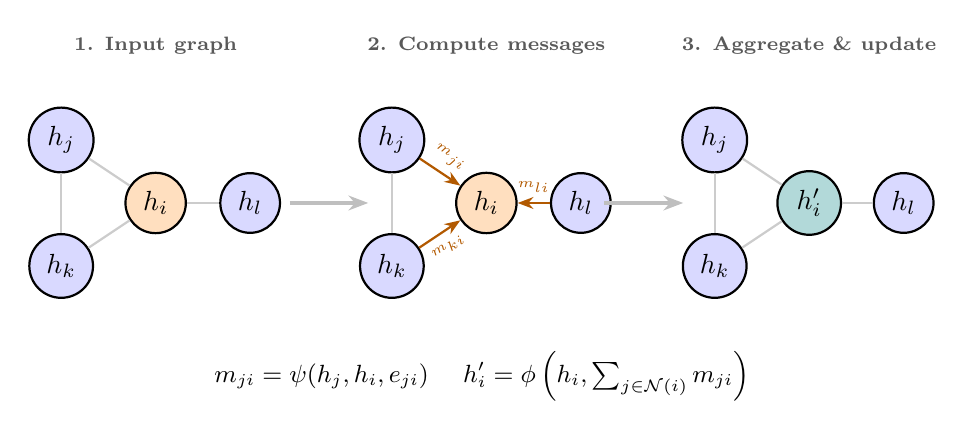
\begin{tikzpicture}[
    node distance=1.2cm,
    gnode/.style={circle, draw, minimum size=0.75cm, thick},
    target/.style={gnode, fill=orange!25},
    neighbor/.style={gnode, fill=blue!15},
    updated/.style={gnode, fill=teal!30},
    msg/.style={-{Stealth[length=2mm]}, thick},
    edge/.style={thick, gray!40},
    arrow/.style={-{Stealth[length=2.5mm]}, very thick},
    label/.style={font=\scriptsize},
    stage/.style={font=\scriptsize\bfseries, text=gray!70!black}
]

% === STAGE 1: INPUT GRAPH ===
\node[stage] at (-4.5, 2) {1. Input graph};

\begin{scope}[shift={(-4.5, 0)}]
    \node[target] (i1) at (0, 0) {$h_i$};
    \node[neighbor] (j1) at (-1.2, 0.8) {$h_j$};
    \node[neighbor] (k1) at (-1.2, -0.8) {$h_k$};
    \node[neighbor] (l1) at (1.2, 0) {$h_l$};

    \draw[edge] (i1) -- (j1);
    \draw[edge] (i1) -- (k1);
    \draw[edge] (i1) -- (l1);
    \draw[edge] (j1) -- (k1);
\end{scope}

% Arrow to stage 2
\draw[arrow, gray!50] (-2.8, 0) -- (-1.8, 0);

% === STAGE 2: COMPUTE MESSAGES ===
\node[stage] at (-0.3, 2) {2. Compute messages};

\begin{scope}[shift={(-0.3, 0)}]
    \node[target] (i2) at (0, 0) {$h_i$};
    \node[neighbor] (j2) at (-1.2, 0.8) {$h_j$};
    \node[neighbor] (k2) at (-1.2, -0.8) {$h_k$};
    \node[neighbor] (l2) at (1.2, 0) {$h_l$};

    \draw[edge] (j2) -- (k2);

    % Message arrows with labels
    \draw[msg, orange!70!black] (j2) -- node[above, sloped, font=\tiny] {$m_{ji}$} (i2);
    \draw[msg, orange!70!black] (k2) -- node[below, sloped, font=\tiny] {$m_{ki}$} (i2);
    \draw[msg, orange!70!black] (l2) -- node[above, font=\tiny] {$m_{li}$} (i2);
\end{scope}

% Arrow to stage 3
\draw[arrow, gray!50] (1.2, 0) -- (2.2, 0);

% === STAGE 3: AGGREGATE & UPDATE ===
\node[stage] at (3.8, 2) {3. Aggregate \& update};

\begin{scope}[shift={(3.8, 0)}]
    \node[updated] (i3) at (0, 0) {$h'_i$};
    \node[neighbor] (j3) at (-1.2, 0.8) {$h_j$};
    \node[neighbor] (k3) at (-1.2, -0.8) {$h_k$};
    \node[neighbor] (l3) at (1.2, 0) {$h_l$};

    \draw[edge] (i3) -- (j3);
    \draw[edge] (i3) -- (k3);
    \draw[edge] (i3) -- (l3);
    \draw[edge] (j3) -- (k3);
\end{scope}

% Equations below
\node[font=\small, align=left] at (-0.3, -2.2) {
$m_{ji} = \psi(h_j, h_i, e_{ji})$ \quad
$h'_i = \phi\left(h_i, \sum_{j \in \mathcal{N}(i)} m_{ji}\right)$
};

\end{tikzpicture}

\caption{Message passing in three stages. (1) Start with node features on a graph. (2) Each node computes messages from its neighbors using a learned function $\psi$. (3) Messages are aggregated (summed) and combined with the node's own features to produce updated representations.}
\label{fig:gnn_detailed}
\end{figure}

\paragraph{A simple message-passing update equation.}
\beq
h_v^{(\ell+1)} = \phi\left( h_v^{(\ell)}, \sum_{u \in \mathcal{N}(v)} \psi(h_u^{(\ell)}, h_v^{(\ell)}, e_{uv}) \right)
\eeq

Unpacking this a bit:
\begin{enumerate}
    \item \textbf{Message}: For each neighbor $u$ of node $v$, compute a message $\psi(h_u, h_v, e_{uv})$. The message depends on sender, receiver, and edge features.
    \item \textbf{Aggregate}: Sum messages over all neighbors. This is where permutation invariance comes from---sum doesn't depend on order.
    \item \textbf{Update}: Combine aggregated messages with the node's current state using $\phi$ to get the new representation.
\end{enumerate}

Both $\psi$ and $\phi$ are learned networks (typically MLPs). The same networks apply to all nodes and edges---\emph{parameter sharing across the graph}.

\paragraph{Hidden dimensions (channels).} Like CNNs, GNNs have a notion of channels: the hidden dimension $d$ of the node representations $h_v \in \R^d$. A node's ``features'' are a $d$-dimensional vector---you can think of each dimension as detecting a different pattern, just like channels in a CNN. More dimensions mean more expressive power but also more parameters.

\paragraph{Connection to Deep Sets and CNNs.} Message passing generalizes both:
\begin{itemize}
    \item \textbf{Deep Sets} is a GNN on a graph with no edges (or a fully-connected graph with uniform edges).
    \item \textbf{CNN} is a GNN on a grid graph where each pixel connects to its spatial neighbors. The kernel weights are the message function.
\end{itemize}

\paragraph{From nodes to graphs.} Message passing produces node representations $h_v$. For graph-level predictions (is this molecule toxic?), \emph{pool} the nodes:
\beq
h_{\mathcal{G}} = \sum_{v \in \mathcal{V}} h_v
\eeq
This is exactly Deep Sets applied to the final node representations.

\paragraph{Graph attention.} Standard message passing treats all neighbors equally (or weights them only by edge features). But different neighbors may have different importance---and the importance may depend on the \emph{content} of the nodes, not just the graph structure.
\textbf{Attention} learns to weight neighbors by relevance:
\beq
h_v' = \sum_{u \in \mathcal{N}(v)} \alpha_{uv} \cdot \psi(h_u)
\eeq

The attention weights $\alpha_{uv}$ are computed from node features:
\beq
\alpha_{uv} = \frac{\exp(f(h_u, h_v))}{\sum_{w \in \mathcal{N}(v)} \exp(f(h_w, h_v))}
\eeq

The scoring function $f$ (typically a small network or inner product) computes how relevant neighbor $u$ is for node $v$. The softmax ensures weights sum to 1.

\begin{figure}[h]
\centering
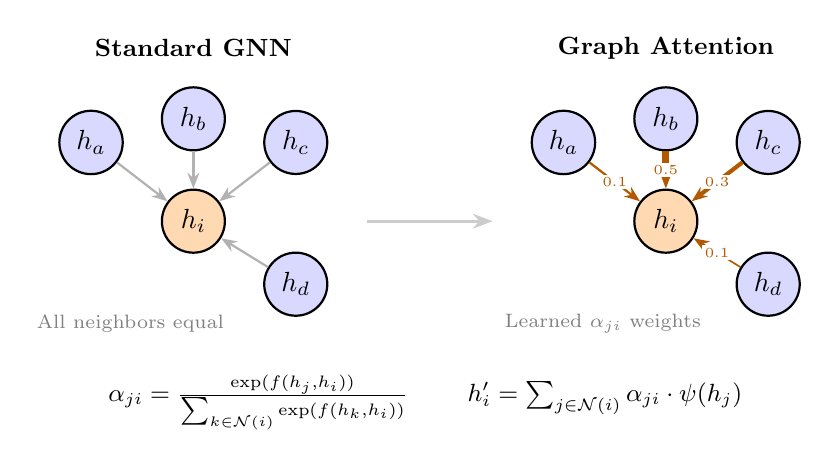
\begin{tikzpicture}[
    node distance=1.0cm,
    gnode/.style={circle, draw, minimum size=0.8cm, thick},
    target/.style={gnode, fill=orange!30},
    neighbor/.style={gnode, fill=blue!15},
    arrow/.style={-{Stealth[length=2.5mm]}, thick},
    attn/.style={-{Stealth[length=2mm]}, thick},
    label/.style={font=\scriptsize},
    weight/.style={font=\tiny, fill=white, inner sep=1pt}
]

% Left side: uniform aggregation
\node[font=\small\bfseries] at (-3, 2.2) {Standard GNN};

\begin{scope}[shift={(-3, 0)}]
    \node[target] (i1) at (0, 0) {$h_i$};
    \node[neighbor] (a1) at (-1.3, 1) {$h_a$};
    \node[neighbor] (b1) at (0, 1.3) {$h_b$};
    \node[neighbor] (c1) at (1.3, 1) {$h_c$};
    \node[neighbor] (d1) at (1.3, -0.8) {$h_d$};

    % Equal thickness arrows
    \draw[attn, gray!60] (a1) -- (i1);
    \draw[attn, gray!60] (b1) -- (i1);
    \draw[attn, gray!60] (c1) -- (i1);
    \draw[attn, gray!60] (d1) -- (i1);

    \node[font=\scriptsize, text=gray] at (-0.8, -1.3) {All neighbors equal};
\end{scope}

% Arrow between
\draw[arrow, very thick, gray!40] (-0.8, 0) -- (0.8, 0);

% Right side: attention-weighted
\node[font=\small\bfseries] at (3, 2.2) {Graph Attention};

\begin{scope}[shift={(3, 0)}]
    \node[target] (i2) at (0, 0) {$h_i$};
    \node[neighbor] (a2) at (-1.3, 1) {$h_a$};
    \node[neighbor] (b2) at (0, 1.3) {$h_b$};
    \node[neighbor] (c2) at (1.3, 1) {$h_c$};
    \node[neighbor] (d2) at (1.3, -0.8) {$h_d$};

    % Variable thickness arrows (attention weights)
    \draw[attn, orange!70!black, line width=0.8pt] (a2) -- node[weight, pos=0.5] {0.1} (i2);
    \draw[attn, orange!70!black, line width=2.5pt] (b2) -- node[weight, pos=0.5] {0.5} (i2);
    \draw[attn, orange!70!black, line width=1.5pt] (c2) -- node[weight, pos=0.5] {0.3} (i2);
    \draw[attn, orange!70!black, line width=0.6pt] (d2) -- node[weight, pos=0.5] {0.1} (i2);

    \node[font=\scriptsize, text=gray] at (-0.8, -1.3) {Learned $\alpha_{ji}$ weights};
\end{scope}

% Equations
\node[font=\small, align=center] at (0, -2.3) {
$\alpha_{ji} = \frac{\exp(f(h_j, h_i))}{\sum_{k \in \mathcal{N}(i)} \exp(f(h_k, h_i))}$
\quad\quad
$h'_i = \sum_{j \in \mathcal{N}(i)} \alpha_{ji} \cdot \psi(h_j)$
};

\end{tikzpicture}

\caption{Graph attention learns which neighbors matter. Left: standard GNN weights all neighbors equally. Right: attention weights neighbors by learned relevance scores $\alpha_{ji}$, allowing the network to focus on the most informative connections.}
\label{fig:graph_attention}
\end{figure}

\paragraph{Why attention helps.} Consider predicting a molecule's reactivity. A carbon atom may have several neighbors, but not all matter equally---the oxygen in a carbonyl group matters more than a distant methyl. Attention learns these patterns from data.

Attention also provides some (limited) interpretability: the learned weights $\alpha_{uv}$ show which neighbors influenced each node's representation.

%%%%%%%%%%%%%%%%%%%%%%%%%%%%%%%%%%%%%%%%%%%%%%%%%%%%%%%%%%%%%%%%%%
\section{Attention as a unifying primitive}
%%%%%%%%%%%%%%%%%%%%%%%%%%%%%%%%%%%%%%%%%%%%%%%%%%%%%%%%%%%%%%%%%%

Attention is a general mechanism that unifies several architectures. The core operation is always the same: compute a weighted combination of inputs. What varies is \emph{which} inputs participate and whether the weights are fixed or content-dependent. Figure~\ref{fig:attention_patterns} illustrates the four main patterns.

\begin{figure}[h]
\centering
% Attention patterns: MLP vs CNN vs GNN vs Transformer
% Requires: \usetikzlibrary{arrows.meta, backgrounds, decorations.pathreplacing, calc}

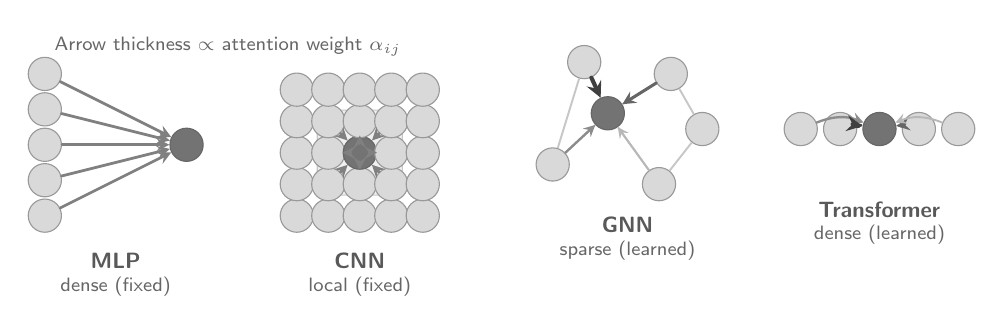
\begin{tikzpicture}[
  node/.style={circle, fill=black!15, draw=black!40, minimum size=12pt, inner sep=0pt},
  query/.style={circle, fill=black!55, draw=black!60, minimum size=12pt, inner sep=0pt},
  edge/.style={-, black!22, line width=0.7pt},
  attn/.style={->, >=stealth, line cap=round},
  panelcap/.style={font=\footnotesize\sffamily, text=black!65},
  panelmicro/.style={font=\scriptsize\sffamily, text=black!60},
]

% Qualitative attention weight levels
\tikzset{
  attnStrong/.style={attn, black!75, line width=1.5pt},
  attnMed/.style={attn, black!60, line width=1.1pt},
  attnWeak/.style={attn, black!45, line width=0.85pt},
  attnFaint/.style={attn, black!28, line width=0.7pt},
  attnFixed/.style={attn, black!50, line width=1.0pt},
}

% Panel anchors (4 panels)
\coordinate (Pmlp) at (0.0,0.55);
\coordinate (Pcnn) at (3.2,0.55);
\coordinate (Pgnn) at (6.4,0.75);
\coordinate (Ptrf) at (9.6,0.95);

% =========================
% MLP (no structure)
% =========================
\begin{scope}[shift={(Pmlp)}]
  % Input layer (5 nodes)
  \foreach \j in {0,1,2,3,4} {
    \node[node] (mlp\j) at (0, \j*0.45) {};
  }
  % Output node (query)
  \node[query] (mlpout) at (1.8, 0.9) {};

  % All-to-one with uniform weights (fixed)
  \foreach \j in {0,1,2,3,4} {
    \draw[attnFixed] (mlp\j) -- (mlpout);
  }

  % Label
  \node[panelcap, anchor=north] at (0.9,-0.35) {\textbf{MLP}};
  \node[panelmicro, anchor=north] at (0.9,-0.65) {dense (fixed)};
\end{scope}

% =========================
% CNN (local fixed)
% =========================
\begin{scope}[shift={(Pcnn)}]
  % 5x5 grid (smaller)
  \foreach \i in {0,1,2,3,4} {
    \foreach \j in {0,1,2,3,4} {
      \ifnum\i=2
        \ifnum\j=2
          \node[query] (cnn\i\j) at (\i*0.4, \j*0.4) {};
        \else
          \node[node] (cnn\i\j) at (\i*0.4, \j*0.4) {};
        \fi
      \else
        \node[node] (cnn\i\j) at (\i*0.4, \j*0.4) {};
      \fi
    }
  }

  % highlight 3x3 receptive field
  \begin{pgfonlayer}{background}
    \draw[rounded corners=2pt, draw=black!22, fill=black!6]
      ($(cnn11)+(-0.14,-0.14)$) rectangle ($(cnn33)+(0.14,0.14)$);
  \end{pgfonlayer}

  % uniform local aggregation (fixed weights)
  \foreach \i in {1,2,3} {
    \foreach \j in {1,2,3} {
      \ifnum\i=2
        \ifnum\j=2\else \draw[attnFixed] (cnn\i\j) -- (cnn22);\fi
      \else
        \draw[attnFixed] (cnn\i\j) -- (cnn22);
      \fi
    }
  }

  % Label
  \node[panelcap, anchor=north] at (0.8,-0.35) {\textbf{CNN}};
  \node[panelmicro, anchor=north] at (0.8,-0.65) {local (fixed)};
\end{scope}

% =========================
% GNN (sparse, content-dependent)
% =========================
\begin{scope}[shift={(Pgnn)}]
  \node[query] (g0) at (0.75, 1.1) {};
  \node[node]  (g1) at (0.05, 0.45) {};
  \node[node]  (g2) at (0.45, 1.75) {};
  \node[node]  (g3) at (1.55, 1.6) {};
  \node[node]  (g4) at (1.4, 0.2) {};
  \node[node]  (g5) at (1.95, 0.9) {};

  % edges (structure)
  \draw[edge] (g0) -- (g1);
  \draw[edge] (g0) -- (g2);
  \draw[edge] (g0) -- (g3);
  \draw[edge] (g0) -- (g4);
  \draw[edge] (g1) -- (g2);
  \draw[edge] (g3) -- (g5);
  \draw[edge] (g4) -- (g5);

  % learned attention weights (varying)
  \draw[attnStrong] (g2) -- (g0);
  \draw[attnMed]    (g3) -- (g0);
  \draw[attnWeak]   (g1) -- (g0);
  \draw[attnFaint]  (g4) -- (g0);

  % Label
  \node[panelcap, anchor=north] at (1.0,-0.1) {\textbf{GNN}};
  \node[panelmicro, anchor=north] at (1.0,-0.4) {sparse (learned)};
\end{scope}

% =========================
% Transformer (dense, content-dependent)
% =========================
\begin{scope}[shift={(Ptrf)}]
  \node[node]  (t0) at (0.0, 0.7) {};
  \node[node]  (t1) at (0.5, 0.7) {};
  \node[query] (t2) at (1.0, 0.7) {};
  \node[node]  (t3) at (1.5, 0.7) {};
  \node[node]  (t4) at (2.0, 0.7) {};

  % dense global attention (varying weights)
  \draw[attnWeak,   bend left=22]  (t0) to (t2);
  \draw[attnStrong, bend left=10]  (t1) to (t2);
  \draw[attnMed,    bend right=10] (t3) to (t2);
  \draw[attnFaint,  bend right=22] (t4) to (t2);

  % Label
  \node[panelcap, anchor=north] at (1.0,-0.1) {\textbf{Transformer}};
  \node[panelmicro, anchor=north] at (1.0,-0.4) {dense (learned)};
\end{scope}

% Arrow weight legend
\node[panelmicro, anchor=west] at (0, 2.7) {Arrow thickness $\propto$ attention weight $\alpha_{ij}$};

\end{tikzpicture}

\caption{Attention patterns across architectures. Dark nodes are queries; arrows show which inputs contribute. \textbf{MLP}: all inputs, fixed weights. \textbf{CNN}: local inputs, fixed weights (same kernel everywhere). \textbf{GNN}: graph neighbors, learned weights. \textbf{Transformer}: all inputs, learned weights. Arrow thickness indicates attention weight.}
\label{fig:attention_patterns}
\end{figure}

\paragraph{The general form.} Given a query $q$, keys $k_1, \ldots, k_n$, and values $v_1, \ldots, v_n$:
\beq
\text{output} = \sum_{i=1}^n \alpha_i \cdot v_i, \quad \text{where} \quad \alpha_i = \frac{\exp(q \cdot k_i)}{\sum_j \exp(q \cdot k_j)}
\eeq
The query asks ``what am I looking for?'' The keys say ``what do I contain?'' The dot product measures relevance. This is \emph{scaled dot-product attention}, the building block of Transformers.

\paragraph{CNNs as fixed local attention.} A convolution computes:
\beq
h_{ij} = \sum_{a,b} W_{ab} \cdot x_{i+a, j+b}
\eeq
This is attention where the weights $W_{ab}$ are fixed (learned once, used everywhere) and the neighborhood is local (only nearby pixels). The ``attention pattern'' is the same at every position---a fixed $3 \times 3$ or $5 \times 5$ window.

\paragraph{GNNs as sparse attention.} Graph attention computes:
\beq
h_v = \sum_{u \in \mathcal{N}(v)} \alpha_{uv} \cdot \psi(h_u)
\eeq
The weights $\alpha_{uv}$ are content-dependent (computed from node features), but attention is restricted to graph neighbors. The graph structure determines \emph{who} can attend to whom; the attention mechanism determines \emph{how much}.

\paragraph{Transformers as dense attention.} Self-attention in Transformers:
\beq
h_i = \sum_{j=1}^n \alpha_{ij} \cdot v_j, \quad \alpha_{ij} = \text{softmax}_j(q_i \cdot k_j / \sqrt{d})
\eeq
Every position attends to every other position. No locality constraint, no predefined graph. The attention weights are entirely learned from content. This is maximally flexible but costs $O(n^2)$ computation.

\paragraph{MLPs as structure-free mixing.} Where do MLPs fit? A fully connected layer computes:
\beq
h_i = \sum_{j=1}^n W_{ij} \cdot x_j
\eeq
Every output depends on every input, with fixed learned weights $W_{ij}$. This is like dense attention but without content-dependence---the ``attention pattern'' is baked into the weights at training time and doesn't adapt to the input. MLPs assume no structure: no locality, no graph, no notion of which inputs should interact. Maximum flexibility, but also maximum data requirements.

\paragraph{The tradeoff.} These four represent different points on a structure-flexibility spectrum:

\begin{center}
\begin{tabular}{lcccc}
\toprule
& \textbf{MLP} & \textbf{Transformer} & \textbf{GNN} & \textbf{CNN} \\
\midrule
Pattern & Dense global & Dense global & Sparse (graph) & Fixed local \\
Weights & Fixed & Content-dep. & Content-dep. & Fixed \\
Connectivity & All pairs & All pairs & Graph neighbors & Grid neighbors \\
Structure assumed & None & Weak & Medium & Strong \\
\bottomrule
\end{tabular}
\end{center}

Reading left to right: MLPs assume no structure (any input can affect any output). Transformers add content-dependent weights that adapt to each input. GNNs restrict connectivity to graph neighbors. CNNs add the strongest prior: local, translation-invariant patterns.

%%%%%%%%%%%%%%%%%%%%%%%%%%%%%%%%%%%%%%%%%%%%%%%%%%%%%%%%%%%%%%%%%%
\section{Why overparameterized networks work}
%%%%%%%%%%%%%%%%%%%%%%%%%%%%%%%%%%%%%%%%%%%%%%%%%%%%%%%%%%%%%%%%%%

Modern neural networks have far more parameters than training examples. A ResNet for ImageNet has 25 million parameters trained on 1.2 million images. Classical statistics says this should overfit catastrophically---with enough parameters, you can memorize the training set and learn nothing generalizable. Yet these networks generalize well. Why?

Traditional learning theory says: more parameters = more ways to fit noise = worse generalization. The optimal model complexity balances fitting the data against overfitting. Add parameters until validation error starts rising.
%
Neural networks violate this. They can \emph{interpolate}---fit the training data perfectly, even with noisy labels---yet still generalize. The test error doesn't explode when you add more parameters past the interpolation threshold. Instead, it often \emph{decreases} (the ``double descent'' phenomenon).

\paragraph{Why interpolation doesn't necessarily overfit.} Among all functions that fit the training data, SGD finds a particular one---and that one tends to be simple.

Think of it geometrically. In high dimensions, the set of parameters that perfectly fit the training data is a large subspace (when you have more parameters than constraints). Within this subspace, there are infinitely many solutions. Some are jagged and complex; others are smooth and simple. SGD, starting from small random weights and taking small steps, tends to find smooth solutions.

\paragraph{Overparameterization smooths the loss landscape.} With more parameters, the loss landscape becomes better-behaved. Instead of one narrow valley, there are many paths to low loss, so optimization is less likely to get stuck. Overparameterized networks tend to find flat minima---regions where the loss is low over a large volume of parameter space---which correspond to simpler functions that generalize better. Good solutions aren't isolated points but form connected regions; you can move between different good solutions without crossing high-loss barriers.

\paragraph{Inductive bias from optimization.} The architecture constrains \emph{what} the network can represent. But the optimizer constrains \emph{which} of those representable functions it actually finds. SGD with small learning rates, starting from small weights, has an implicit bias toward simpler functions. This ``implicit regularization'' is as important as the explicit architecture. (We'll come back to this when discussing symmetry-based architectures.)

\paragraph{What this means in practice.} Don't fear overparameterization. A network with 10$\times$ more parameters than data points may generalize better than a smaller one---if trained properly. The combination of architecture (encoding the right symmetries) and optimization (finding smooth solutions) produces good generalization even in the overparameterized regime.

%%%%%%%%%%%%%%%%%%%%%%%%%%%%%%%%%%%%%%%%%%%%%%%%%%%%%%%%%%%%%%%%%%
\appendix
\section{The QM9 dataset}
\label{app:qm9}
%%%%%%%%%%%%%%%%%%%%%%%%%%%%%%%%%%%%%%%%%%%%%%%%%%%%%%%%%%%%%%%%%%

QM9 is a benchmark dataset of 134,000 small organic molecules with quantum-mechanical properties computed from density functional theory (DFT). Each molecule contains up to 9 heavy atoms (C, N, O, F) plus hydrogens. The dataset provides a concrete example of molecular property prediction: given a molecule's structure, predict its quantum properties without expensive DFT calculations.

\paragraph{Molecules as graphs.} A molecule is naturally represented as a graph: atoms are nodes, chemical bonds are edges. This is the input to a GNN. Figure~\ref{fig:qm9_graph} shows the concrete representation.

\begin{figure}[h]
\centering
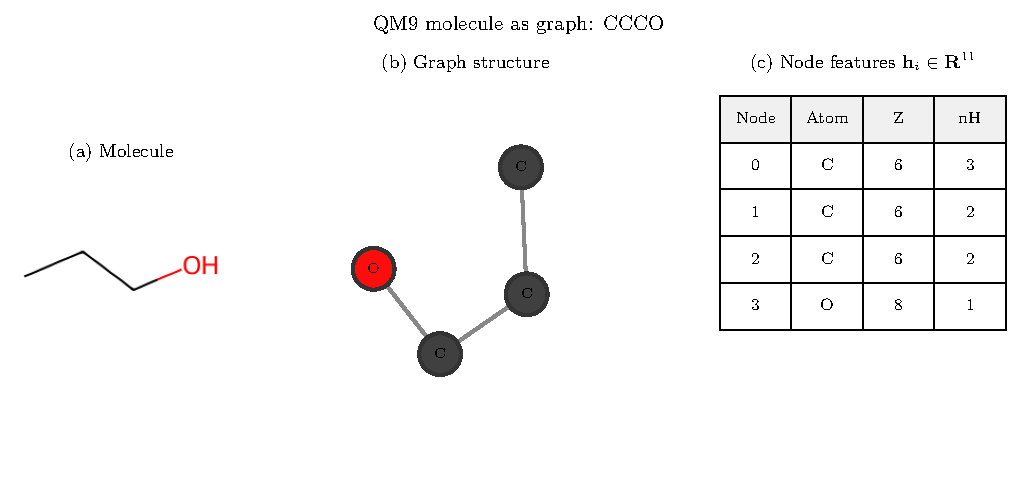
\includegraphics[width=\textwidth]{figures/qm9_graph_structure.pdf}
\caption{QM9 data representation. (a) A molecule visualized with RDKit. (b) The same molecule as a graph: heavy atoms are nodes, bonds are edges. Hydrogens are implicit---encoded in the nH feature rather than as explicit nodes. (c) Each node has an 11-dimensional feature vector; nH indicates the number of attached hydrogens.}
\label{fig:qm9_graph}
\end{figure}

\paragraph{Node features.} Each atom is represented by an 11-dimensional feature vector:
\begin{center}
\begin{tabular}{lll}
\toprule
\textbf{Indices} & \textbf{Feature} & \textbf{Description} \\
\midrule
0--4 & Atom type & One-hot encoding (H, C, N, O, F) \\
5 & Atomic number & Integer (1, 6, 7, 8, 9) \\
6--8 & Hybridization & One-hot (sp, sp$^2$, sp$^3$) \\
9 & Aromatic & Binary (0 or 1) \\
10 & Hydrogen count & Number of attached hydrogens \\
\bottomrule
\end{tabular}
\end{center}

\paragraph{Edge features.} Each bond has a 4-dimensional feature vector: a one-hot encoding of bond type (single, double, triple, aromatic). Edges are stored bidirectionally---each bond $(i,j)$ appears twice as directed edges $i \to j$ and $j \to i$.

\paragraph{Target properties.} QM9 provides 19 quantum-mechanical properties for each molecule, including:
\begin{itemize}
    \item \textbf{HOMO/LUMO energies}: Frontier orbital energies (eV)
    \item \textbf{HOMO-LUMO gap}: Electronic excitation energy (eV)
    \item \textbf{Dipole moment}: Molecular polarity (Debye)
    \item \textbf{Polarizability}: Response to electric field (Bohr$^3$)
    \item \textbf{Thermodynamic properties}: Internal energy, enthalpy, free energy, heat capacity
\end{itemize}
These properties determine a molecule's electronic, optical, and thermodynamic behavior. Predicting them from structure alone---bypassing expensive DFT calculations---is the goal of molecular property prediction.

QM9 is small enough to train on quickly but rich enough to benchmark different architectures.This makes QM9 a good benchmark for comparing how different inductive biases affect learning on the same underlying data.

\end{document}
